% slides.tex
\documentclass[20pt]{beamer}
\usepackage{listings}
\usepackage[utf8]{inputenc}
\usepackage{color}
\usepackage{graphicx}

\usetheme{default}
\usecolortheme{dove}
\useoutertheme{default}

% Slightly smaller title
\setbeamerfont{frametitle}{size=\large}
\setbeamerfont{verb}{size=\small}

% lst settings
\lstset{
    language=Haskell,
    basicstyle=\small,
    gobble=4
}

\newcommand{\vspaced}{
    \vspace{5mm}
}

\begin{document}

\title{BlazeHtml}
\subtitle{Blazingly fast HTML combinators}
\author{Jasper Van der Jeugt}
\date{March 18, 2011}

\begin{frame}[plain]
    \titlepage
\end{frame}

% Introduction
% ------------

\begin{frame}{Hello!}
    My name is Jasper \\
    Student at UGent \\
    I write Haskell \\
    GhentFPG organizer \\
    \texttt{@jaspervdj} \\
    \texttt{jaspervdj.be}
    \begin{picture}(0.0, 0.0)
    \put(40.0, -15.0){
\includegraphics[width=0.5\textwidth]{images/hat.pdf}}
    \end{picture}
\end{frame}

\begin{frame}{Overview}
    \textbf{Introduction} \\
    Why Haskell? \\
    Haskell web frameworks \\
    Case study: BlazeHtml
\end{frame}

% Why Haskell?
% ------------

\begin{frame}{Overview}
    Introduction \\
    \textbf{Why Haskell?} \\
    Haskell web frameworks \\
    Case study: BlazeHtml
\end{frame}

\begin{frame}{Web development: languages used}
    PHP \\
    Ruby \\
    Python
    % TODO: pic
\end{frame}

\begin{frame}{Haskell has an edge}
    Type-safe \\
    Stateless \\
    Compiled \\
    Highly scalable
    % TODO: lambda pic
\end{frame}

\begin{frame}[t, fragile]{Type safety}
    \vspaced
    Is this function error-prone?
    \begin{lstlisting}
    makeImage ::
        Int -> Int -> Image
    \end{lstlisting}
    % TODO: Image width/height
\end{frame}

\begin{frame}[fragile]{Type safety}
    Can prevent many errors
    \begin{lstlisting}
    newtype Width = Width Int
    newtype Height = Height Int
    makeImage ::
        Width -> Height -> Image
    \end{lstlisting}
\end{frame}

\begin{frame}{Pure code}
    Explicit separation of pure and impure code \\
    \vspaced
    \begin{tabular}{l|l}
        Pure         & Impure \\
        Heavens      & Earth  \\
        "Functional" & "Imperative"
    \end{tabular}
    \newline
    \vspaced

    Impure code can call pure code, but not vice versa
\end{frame}

% Haskell web frameworks/libraries
% --------------------------------

\begin{frame}{Overview}
    Introduction \\
    Why Haskell? \\
    \textbf{Haskell web frameworks} \\
    Case study: BlazeHtml
\end{frame}

\begin{frame}[fragile]{General web programming}
    Something like
    \begin{lstlisting}
    app :: Request -> Response
    \end{lstlisting}

    \vspaced
    Or rather
    \begin{lstlisting}
    app :: Request -> IO Response
    \end{lstlisting}
\end{frame}

\begin{frame}[fragile]{Routes}
    Web framework provides routing, e.g.

    \begin{lstlisting}
    route
      [ ("",          root)
      , ("user/:id",  user)
      , ("tweet/:id", tweet)
      ]
    \end{lstlisting}
\end{frame}

\begin{frame}[fragile]{Monadic handlers}
    Implementation of handlers:

    \begin{lstlisting}
      user = do
        id' <- getParam "id"
        user <- getFromDataBase id'
        -- Perform pure operations
        save user
        set reponse
    \end{lstlisting}
\end{frame}

\begin{frame}{WAI}
    \textbf{W}eb \textbf{A}pplication \textbf{I}nterface \\
    Connects server backend to application \\
    Similar to Rack (Ruby) \\
\end{frame}

\begin{frame}{Happstack}
    Has been around since 2003 \\
    Very mature \\
    Complete stack \\
    Yet flexible
\end{frame}

\begin{frame}{Yesod}
    Built on \emph{WAI} \\
    Very high-level \\
    Tightly integrated components \\
    Focus on DSL's \\
\end{frame}

\begin{frame}{Snap Framework}
    Relatively new \\
    Sensible and clean \\
    Fast and highly concurrent \\
    Aims to be a complete framework \\
\end{frame}

\begin{frame}{Warp}
    A very fast web server \\
    Handles 190k req/s \\
    Simple (500 loc) \\
    Backend for \emph{WAI} \\
\end{frame}

% Case study: BlazeHtml
% ---------------------

\begin{frame}{Overview}
    Introduction \\
    Why Haskell? \\
    Haskell web frameworks \\
    \textbf{Case study: BlazeHtml} \\
\end{frame}

\begin{frame}{Webapp architecture}
    HTML generation \\
    Web application server \\
    Data storage layer
\end{frame}

\begin{frame}{BlazeHtml}
    Embedded in Haskell \\
    Efficient Unicode support \\
    Supports HTML 4 and HTML 5 \\
    Pretty fast \\
    Google Summer of Code 2010 \\
    By Simon Meier \& me
\end{frame}

\begin{frame}[fragile]{Example}
    \begin{lstlisting}
    head $ do
        title "Title"
    body $ do
        div ! class_ "fancy" $ do
            "Literal"
        div ! id "info" $ do
            p "Content..."
            p "More..."
    \end{lstlisting}
\end{frame}

\begin{frame}[fragile]{Build your own abstractions}
    \begin{lstlisting}
    includeJS source =
     script ! type_ "text/javascript"
            ! src source
            $ mempty

    includeJS "jquery.min.js"
    \end{lstlisting}
\end{frame}

\begin{frame}[fragile]{HTML representation}
    \begin{lstlisting}
    data Tree a
        = Node a (Tree a) (Tree a)
        | Empty
    \end{lstlisting}
    \vspaced
    A simple, immutable data structure
\end{frame}

\begin{frame}{HTML is a tree}
    Picture here
    % TODO: Html tree picture
\end{frame}

\begin{frame}{Rendering}
    Basically, flattening the tree to some string type
    % TODO: Html -> String picture
\end{frame}

\begin{frame}[fragile]{Concatenating}
    StringBuilder:
    \begin{lstlisting}[language=Java]
    builder.append(someString)
    \end{lstlisting}
    \vspaced

    Builder monoid
    \begin{lstlisting}[language=Java]
    builder1 `mappend` builder2
    \end{lstlisting}
\end{frame}

\begin{frame}[fragile]{Builder Monoid}
    Simple interface:
    \vspaced
    \begin{lstlisting}
    mempty ::
       Builder

    mappend ::
       Builder -> Builder -> Builder
    \end{lstlisting}
\end{frame}

\begin{frame}[fragile]{Implementation}
    % TODO: Builder pic
    Pic here
\end{frame}

\begin{frame}[fragile, b]{BigTable benchmark}
    \begin{lstlisting}
    bigTable :: Html
    bigTable = table $
      forM_ [1 .. 1000] $ \r -> tr $
        forM_ [1 .. 10] $ \c -> td $
          toHtml $ show (row, col)
    \end{lstlisting}
    \vspaced
\end{frame}

\begin{frame}{BigTable benchmark}
    \begin{center}
    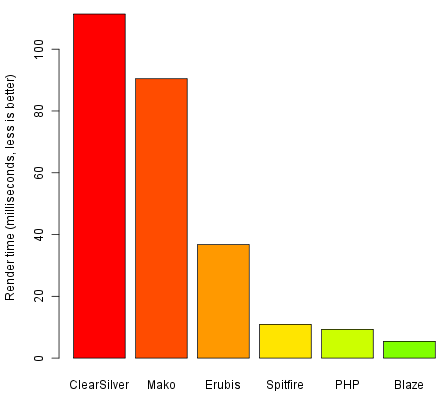
\includegraphics[width=0.8\textwidth]{images/benchmarks.png}
    \end{center}
\end{frame}

\begin{frame}{Questions?}

\end{frame}

\end{document}
